%!TEX root = ../dissertation.tex
% For an example of a full page figure, see Fig.~\ref{fig:myFullPageFigure}.

\chapter{Contesto aziendale}

\section{L'azienda}
Lo stage si è svolto presso l'azienda Pietro Fiorentini S.p.A nella sede principale di Arcugnano. Pietro Fiorentini realizza prodotti e servizi tecnologicamente avanzati per la distribuzione e l'utilizzo del petrolio e del gas naturale a livello globale, con undici stabilimenti nel mondo.

Durante i sui 70 anni di esperienza, l'azienda ha sempre puntato al rinnovamento e alla ricerca di un costante progresso. Pietro fiorentini lavora in un contesto Kaizen ispirato alla filosofia di business nata in Giappone negli anni '80. Kaizen significa miglioramento continuo e indica 5 passi da seguire per avere un metodo sistematico e ripetibile per l'ottimizzazione degli standard di lavoro, questi 5 passi chiamati anche le "5S del Kaizen" sono separare, sistemare, spazzare, standardizzare e sostenere. Questa metodologia spinge verso un atteggiamento di miglioramento continuo dove ogni giorno vengono effettuate piccole migliorie e scoperte altre inefficienze o sprechi.

L'azienda realizza prodotti come valvole, filtri, regolatori di pressione e strumenti di misura, sia per impianti in superficie che subacquei. L'installazione degli strumenti, in particolare per impianti di estrazione subacquei in mare aperto o nell'oceano richiede molte settimane di lavoro e il noleggio di navi apposite per un costo totale di milioni di euro. Per questo motivo poter sapere lo stato di salute e prevedere i malfunzionamenti in uno strumento che deve funzionare isolato per decine di anni è molto importante per l'azienda. A questo proposito il reparto di ricerca e sviluppo sta quindi valutando l'utilizzo di algoritmi di machine learning per il riconoscimento delle anomalie nei propri strumenti. 

Lo stage si è interessato in particolare a una tipologia di strumenti prodotti dalla Pietro Fiorentini: i Multiphase Flow Meter.


\section{Multiphase Flow Meter} \label{multiphaseflowmeter}
Un Multiphase Flow Meter, o MPFM in breve, è un dispositivo utilizzato per misurare le singole portate delle fasi costitutive di un determinato flusso. In questo caso il flusso è una miscela di petrolio, acqua e gas creata durante il processo di estrazione dal pozzo petrolifero.
I MPFM prodotti dalla Pietro Fiorentini sono strumenti non intrusivi per effettuare misurazioni in tempo reale del flusso evitando l'uso di sistemi basati sulla separazione delle diverse fasi.
Gli MPFM sono modulari e possono essere installati in diverse configurazioni, ogni modulo si occupa di effettuare una o più misurazioni sul flusso.

\begin{figure}
	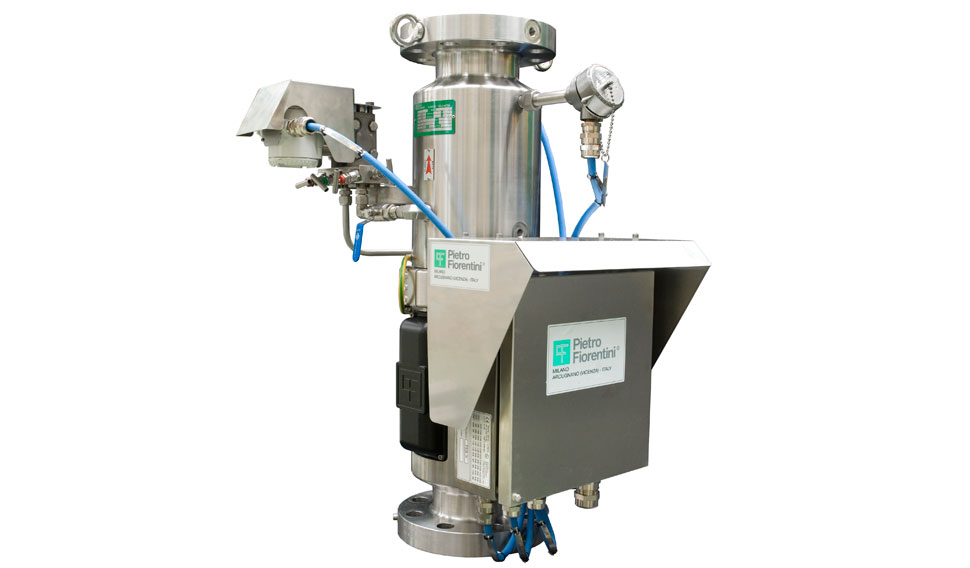
\includegraphics[width=\textwidth]{figures/mpfm}
	\caption[Multiphase Flow Meter]{
		Flowatch 3I, uno dei modelli di Multiphase Flow Meter prodotti da Pietro Fiorentini
		\label{fig:mpfm}}
\end{figure}


La misurazione dei flussi multifase è un problema complesso e richiede la considerazione di molte possibili condizioni. In particolare ci sono molti regimi di scorrimento del flusso a seconda della velocità delle parti liquide e gassose \cite{multiphaseIntroduction}.

I principali regimi di scorrimento sono:

\begin{itemize}
	\item{Bubble}: il gas è sospeso in bollicine all'interno del liquido, accade quando la parte liquida è più veloce di quella gassosa.
	\item{Finely dispersed bubble}: il gas è sospeso in bollicine molto piccole all'interno del liquido.
	\item{Slug}: il flusso è a intermittenza prevalentemente liquido e prevalentemente gassoso, formando delle grosse bolle di gas.
	\item{Churn}: all'aumentare della velocità del gas il flusso diventa irregolare e la parte liquida sale e scende continuamente.
	\item{Annular}: ad alte velocità del gas la parte liquida forma un anello intorno alle pareti della tubatura, e il gas scorre nel centro.
\end{itemize}

\begin{figure}
	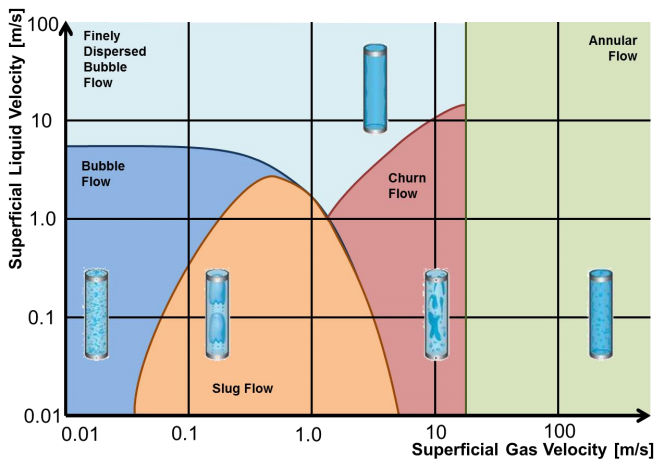
\includegraphics[width=\textwidth]{figures/flowtypes}
	\caption[Tipologie di flusso multifase]{
		I principali regimi di scorrimento del flusso multifase in base alla velocità della parte liquida e della parte gassosa \cite{multiphaseIntroduction}.
		\label{fig:flowtypes}}
\end{figure}

L'irregolarità del flusso rende anche più difficile il riconoscimento delle anomalie nel funzionamento dello strumento. Dei valori che a prima vista sembrano anomali potrebbero semplicemente essere delle bolle più grosse di gas, oppure il passaggio improvviso a un altro regime di scorrimento. In questi casi le anomalie registrate fanno parte del funzionamento corretto dello strumento e non devono essere quindi considerati come valori anormali.

\section{Struttura dei dati} \label{"StrutturaDeiDati"}
I dati rilevanti al progetto riguardano una serie di test effettuati in vari laboratori negli ultimi dieci anni. I test consistono nell'uso di un Multiphase Flow Meter in un circuito chiuso, in modo da poter controllare accuratamente la composizione e le condizioni del flusso che viene fatto circolare. 

Durante il test si registrano le letture di tutti i sensori presenti nel MPFM, questi dati vengono quindi salvati in file singoli, ognuno dei quali contiene in genere un minuto di lettura. I file sono in formato proprietario BIN o BIX e rappresentano i dati nel loro stato "raw", ad esempio un sensore che misura la pressione non salverà direttamente dei valori in atmosfere ma potrebbe salvare dei voltaggi che dovranno essere a loro volta interpretati.

Le informazioni sulla configurazione del MPFM e sulle condizioni del flusso non sono salvate nei file raw, sono salvate invece in file separati, rispettivamente un file di testo per la configurazione del MPFM e un foglio di calcolo per le condizioni del flusso. Questo foglio di calcolo, chiamato anche foglio di riferimento, rappresenta quindi le condizioni in cui sono state effettuate le letture dei sensori, in particolare descrive le seguenti proprietà del flusso per ogni file raw:

\begin{itemize}
	\item \bfseries{Qgas}: Il volume della componente di gas nel flusso
	\item \bfseries{Qwater}: Il volume della componente d'acqua nel flusso
	\item \bfseries{Qwater}: Il volume della componente di petrolio nel flusso
	\item \bfseries{WLR}: Water Liquid Ratio, la percentuale di acqua sul totale del liquido. Calcolato con la formula: \[\frac{Qwater}{Qwater+Qoil}\]
	\item \bfseries{GVF}: Gas Volume Fraction, la frazione di gas sul volume totale. Calcolato con la formula: \[\frac{Qgas}{Qwater+Qoil+Qgas}\]
	\item \bfseries{Pressure}: La pressione del flusso
	\item \bfseries{Temperature}: La temperatura del flusso
\end{itemize}




%% Requires fltpage2 package
%%
% \begin{FPfigure}
% 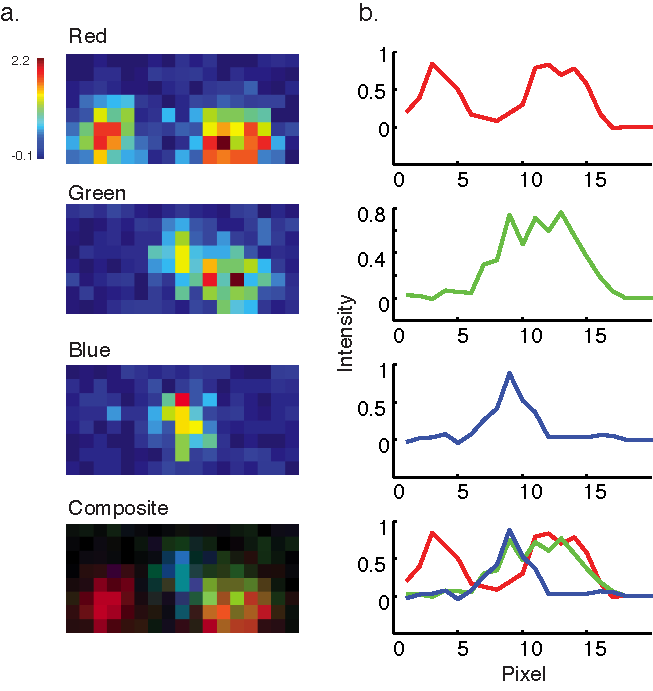
\includegraphics[width=\textwidth]{figures/fullpage}
% \caption[Short figure name.]{This is a full page figure using the FPfigure command. It takes up the whole page and the caption appears on the preceding page. Its useful for large figures. Harvard's rules about full page figures are tricky, but you don't have to worry about it because we took care of it for you. For example, the full figure is supposed to have a title in the same style as the caption but without the actual caption. The caption is supposed to appear alone on the preceding page with no other text. You do't have to worry about any of that. We have modified the fltpage package to make it work. This is a lengthy caption and it clearly would not fit on the same page as the figure. Note that you should only use the FPfigure command in instances where the figure really is too large. If the figure is small enough to fit by the caption than it does not produce the desired effect. Good luck with your thesis. I have to keep writing this to make the caption really long. LaTex is a lot of fun. You will enjoy working with it. Good luck on your post doctoral life! I am looking forward to mine. \label{fig:myFullPageFigure}}
% \end{FPfigure}
% \afterpage{\clearpage}
